% ============================================================================
% marin-spin poster  —  AI-in-Chemistry conference
% Landscape 36 x 24 in (US-standard, ~A1 area).  3 columns.  beamerposter.
%
% Build:  pdflatex poster.tex   (or lualatex)   — needs the `beamerposter` pkg.
% Figures: drop PNGs in ./figures/ (see \includegraphics paths + the mapping
% from scratch/ noted in chat). [TODO] marks results still being finalized.
%
% Orientation/size knob: change the \usepackage[...]{beamerposter} line below.
%   landscape 36x24:  width=91.44,height=60.96   (current)
%   portrait  24x36:  orientation=portrait,width=60.96,height=91.44
% ============================================================================
\documentclass[final]{beamer}
% Portrait 36 x 48 in (91.44 x 121.92 cm).  2 columns.
\usepackage[orientation=portrait,size=custom,width=91.44,height=121.92,scale=1.08]{beamerposter}
\usepackage[T1]{fontenc}
\usepackage{graphicx}
\usepackage{booktabs}
\usepackage{amsmath,amssymb}
\usepackage{relsize}   % \mathlarger to enlarge the summation operator
\usepackage{xcolor}
% Lato (the Open Athena blog font, sans-serif) for text; newtxmath for math symbols.
% professionalfonts keeps beamer from mis-sizing large operators (\sum blank/tiny).
\usefonttheme{professionalfonts}
\usepackage[default]{lato}
\usepackage{newtxmath}

% ---- Open Athena palette (sampled from the OA brand deck) --------------------
\definecolor{ink}{HTML}{2E2C28}        % charcoal text
\definecolor{oabrown}{HTML}{7B583A}    % deep brown
\definecolor{oaterra}{HTML}{A0734C}    % terracotta (primary accent)
\definecolor{oasage}{HTML}{696751}     % sage / olive
\definecolor{oapaper}{HTML}{BDB1A5}    % warm taupe (brand field)
\definecolor{oacream}{HTML}{F2EDE6}    % light cream (block bodies)
\definecolor{oablue}{HTML}{0F4C81}     % MarinSpin blue (from the plots) --- citation markers

\setbeamercolor{background canvas}{bg=oapaper}
\setbeamercolor{block title}{fg=white,bg=oaterra}
\setbeamercolor{block body}{fg=ink,bg=oacream}
\setbeamercolor{headline}{fg=ink,bg=oapaper}
\setbeamertemplate{blocks}[rounded][shadow=false]
\addtobeamertemplate{block end}{}{\vspace{0.5\baselineskip}}  % airier spacing between blocks
\setbeamertemplate{navigation symbols}{}
\setbeamerfont{block title}{size=\large,series=\bfseries}
\setbeamercolor{itemize item}{fg=oasage}
\setbeamercolor{itemize subitem}{fg=oasage}
\hypersetup{colorlinks=true,urlcolor=oaterra}

% Unify all bold emphasis to brand brown (so \keypt and \textbf labels match).
\newcommand{\keypt}[1]{\textcolor{oabrown}{\textbf{#1}}}
% Reference markers: blue superscript so they don't read as math exponents.
\newcommand{\refcite}[1]{\textsuperscript{\textcolor{oablue}{#1}}}
\let\origtextbf\textbf
\renewcommand{\textbf}[1]{\textcolor{oabrown}{\origtextbf{#1}}}

% Airier text: looser line spacing + more space between bullets/paragraphs.
\linespread{1.2}
\setlength{\parskip}{0.5\baselineskip}
\makeatletter
\def\@listi{\leftmargin\leftmargini \topsep 4pt \parsep 0pt \itemsep 0.6\baselineskip}
\let\@listI\@listi
\makeatother

\title{Can a Transformer Learn Coarsening Dynamics?}
\author{}
\begin{document}

% ---- HEADLINE ---------------------------------------------------------------
\begin{frame}[t]
\begin{beamercolorbox}[wd=\paperwidth,sep=18pt]{headline}
  \begin{minipage}[c]{0.165\paperwidth}
    \sbox0{\color{ink}\bfseries\shortstack[l]{{\veryHuge Open}\\[4pt]{\veryHuge Athena}}}%
    \usebox0\hspace{8pt}%
    \raisebox{\dimexpr-0.2\ht0-1.2\dp0\relax}{
\includegraphics[height=\dimexpr1.4\ht0+1.4\dp0\relax]{figures/oa_tree.png}}%
  \end{minipage}\hfill
  \begin{minipage}[c]{0.805\paperwidth}
    \centering
    {\veryHuge\bfseries MarinSpin: Can a Transformer Learn Coarsening Dynamics?}\\[10pt]
    {\Large Reproducing 2D-Ising kinetic Monte-Carlo \emph{rates and waiting times} from trajectory data alone}\\[8pt]
    {\large Y.~Elmatad \quad R.~Wojdyla \quad D.~Hall \qquad \textbf{Open Athena} \qquad Built on \textbf{Marin} \;\textbar\; \href{https://marin.community/}{\texttt{marin.community}} \qquad \texttt{yael.elmatad@openathena.ai}}
  \end{minipage}
\end{beamercolorbox}
{\color{oaterra}\rule{\paperwidth}{5pt}}
\vspace{10pt}

% ---- TAKEAWAYS banner (full width, directly under the title) ----------------
\begin{columns}
\begin{column}{0.97\paperwidth}
  \begin{block}{Takeaways}
    \begin{columns}[t,onlytextwidth]
      \begin{column}{0.305\paperwidth}
        \keypt{Learns kinetic Monte Carlo (KMC) from data.} A vanilla transformer recovers flip
        \emph{rates} and \emph{waiting times} from trajectories alone.
      \end{column}
      \begin{column}{0.305\paperwidth}
        \keypt{Grammar matters.} MarinSpin is off-the-shelf; much of the modeling work lives in
        the \emph{tokenization \& grammar}.
      \end{column}
      \begin{column}{0.305\paperwidth}
        \keypt{Matches the true dynamics.} Per-step KL near the oracle floor; reproduces $\xi(T)$
        across $T_c$ and coarsening under rollout.
      \end{column}
    \end{columns}
  \end{block}
\end{column}
\end{columns}
\vspace{6pt}

\begin{columns}[t]

% ======================= LEFT COLUMN ========================================
\begin{column}{.48\paperwidth}

  \begin{block}{Goal \& Strategy}
    \keypt{Goal:} model the \emph{dynamics} of systems whose governing rules are \emph{generally
    unknown}.

    \medskip
    \keypt{Strategy:} establish the method on a system where the ground truth \emph{is} known ---
    the 2D-Ising model, where a learned model can be scored against the \emph{exact} transition rates.
  \end{block}

  \begin{block}{The 2D Ising model}
    Spins $s_i=\pm1$ on a lattice with energy (Hamiltonian) $\mathcal{H}=-J\sum_{\langle ij\rangle} s_i s_j$
    (we set $J{=}1$), where $\langle ij\rangle$ runs over \emph{nearest-neighbour} pairs. It is the \keypt{canonical model of phase
    transitions and coarsening}\refcite{3}: below a critical temperature $T_c\approx2.27$ it orders into
    growing domains, above $T_c$ it is disordered.
  \end{block}

  \begin{block}{System \& data}
    2D Ising, $L{\times}L$ lattice ($L{=}16$), periodic; temperature $T$.
    \textbf{Rejection-free KMC}\refcite{1}: flipping site $i$ changes the energy by $\Delta E_i$ and has rate
    $w_i=\min(1,e^{-\Delta E_i/T})$\refcite{2}; pick site $i$ with probability $w_i/R$ (total rate $R=\sum_i w_i$)
    and advance the clock by waiting time $\Delta t\sim\mathrm{Exp}(R)$.

    \medskip
    \textbf{Tokenization.} Vocabulary: a $T$-bin per temperature, two spin tokens
    ($\uparrow,\downarrow$), $N{=}L^2$ position tokens, and log-binned $\Delta t$ tokens. A window of $W$
    events tokenizes as:
    \par\smallskip
    {\centering$[\,T\,]\;\underbrace{[\,\text{initial config tokens}\,]}_{\times\,2}\;\underbrace{[\,T\,][\,\mathrm{pos}\,][\,\Delta t\,]}_{\times\,W}$\par}\smallskip
    \textbf{Example} ($2{\times}2$):
    \par\smallskip
    {\centering$[\,T{=}1.5\,]\ \underbrace{[\mathrm{pos}_0][{\uparrow}][\mathrm{pos}_1][{\downarrow}][\mathrm{pos}_2][{\downarrow}][\mathrm{pos}_3][{\uparrow}]}_{\text{config, written twice}}\ [\,T{=}1.5\,][\mathrm{pos}_3][\Delta t{=}0.4]\ [\,T{=}1.5\,][\mathrm{pos}_1][\Delta t{=}1.2]$\par}\smallskip

    \medskip
    \textbf{Data.} 14 discrete $T$: 6 cold $[1.5,2.0]$ + 8 hot $[2.8,3.5]$; \keypt{critical window
    $(2.0,2.8)$ around $T_c$ held out}. Trajectories equilibrated to steady magnetization $|m|=|\tfrac{1}{N}\sum_i s_i|$ before recording.
  \end{block}

  \begin{block}{Model \& training}
    \begin{itemize}
      \item \textbf{Architecture:} an \keypt{off-the-shelf decoder-only transformer}\refcite{4} (GPT-style,
            with rotary position embeddings, RoPE\refcite{5}). $d_{\rm model}$=256,
            6 layers, 8 heads, feed-forward width 1024; vocab $\approx$339; context 1280;
            \keypt{$\sim$5\,M parameters}.
      \item \textbf{Objective:} next-token cross-entropy on the (pos, $\Delta t$) event tokens only.
      \item \textbf{Data:} 70{,}000 KMC trajectories (14 temperatures $\times$ 5{,}000), 500 events each
            $\Rightarrow\ \sim$0.7\,M training windows.
      \item \textbf{Training:} $\sim$18 epochs, batch 256, AdamW, lr $10^{-3}$ cosine,
            \keypt{fp32} --- $\sim$6.7\,h on a single \keypt{TPU v6e-4} (4 chips).
    \end{itemize}
  \end{block}

  \begin{block}{Built on Marin}
    \begin{minipage}[t]{\dimexpr\linewidth-3.6cm\relax}\vspace{0pt}
      \keypt{Marin} (\href{https://marin.community/}{marin.community}) is an open lab for building
      foundation models openly. MarinSpin uses its model \& training stack.
    \end{minipage}\hfill
    \begin{minipage}[t]{3cm}\vspace{0pt}
      
\includegraphics[width=3cm]{figures/qr_marin.png}
    \end{minipage}
  \end{block}

  \begin{block}{$\Delta t$ tokens \& autoregressive rollout}
    \textbf{Waiting-time tokens.} The continuous $\Delta t\sim\mathrm{Exp}(R)$ is quantized into
    log-spaced bins ($+$ under/overflow); MarinSpin predicts a \emph{category} over $\Delta t$-bins.

    \medskip
    \textbf{Rollout.} Autoregressive, one event at a time: from the current config MarinSpin emits
    $p(\text{flip site})\to$ sample $i$, then $p(\Delta t)\to$ sample a bin and draw $\Delta t$
    log-uniformly within it; flip spin $i$, advance the clock by $\Delta t$, append, repeat.
  \end{block}

  \begin{block}{The oracle floor}
    The dynamics are \emph{stochastic}, so the cross-entropy decomposes as
    \[
      \mathcal{L} \;=\; \underbrace{S(p_{\rm KMC})}_{\text{oracle floor}}
      \;+\; D_{\mathrm{KL}}\!\big(p_{\rm KMC}\,\Vert\,q_{\rm model}\big).
    \]
    for true dynamics $p_{\rm KMC}$ and model $q_{\rm model}$. The \keypt{oracle floor} is the
    conditional Shannon entropy of the true dynamics; the \keypt{Kullback--Leibler divergence
    $D_{\mathrm{KL}}$} is the residual loss:

    \medskip
    \centering
    \begin{tabular}{lcc}
      \toprule
       & $T{=}1.5$ (cold) & $T{=}3.5$ (hot)\\
      \midrule
      oracle floor $S$ (nats)              & 3.435 & 4.274\\
      MarinSpin loss $\mathcal{L}$         & 3.43  & 4.30\\
      residual $D_{\mathrm{KL}}$           & 0.012 & 0.038\\
      \bottomrule
    \end{tabular}
  \end{block}

  \begin{block}{Out of distribution (OOD) quench reproduces coarsening dynamics}
    \centering
    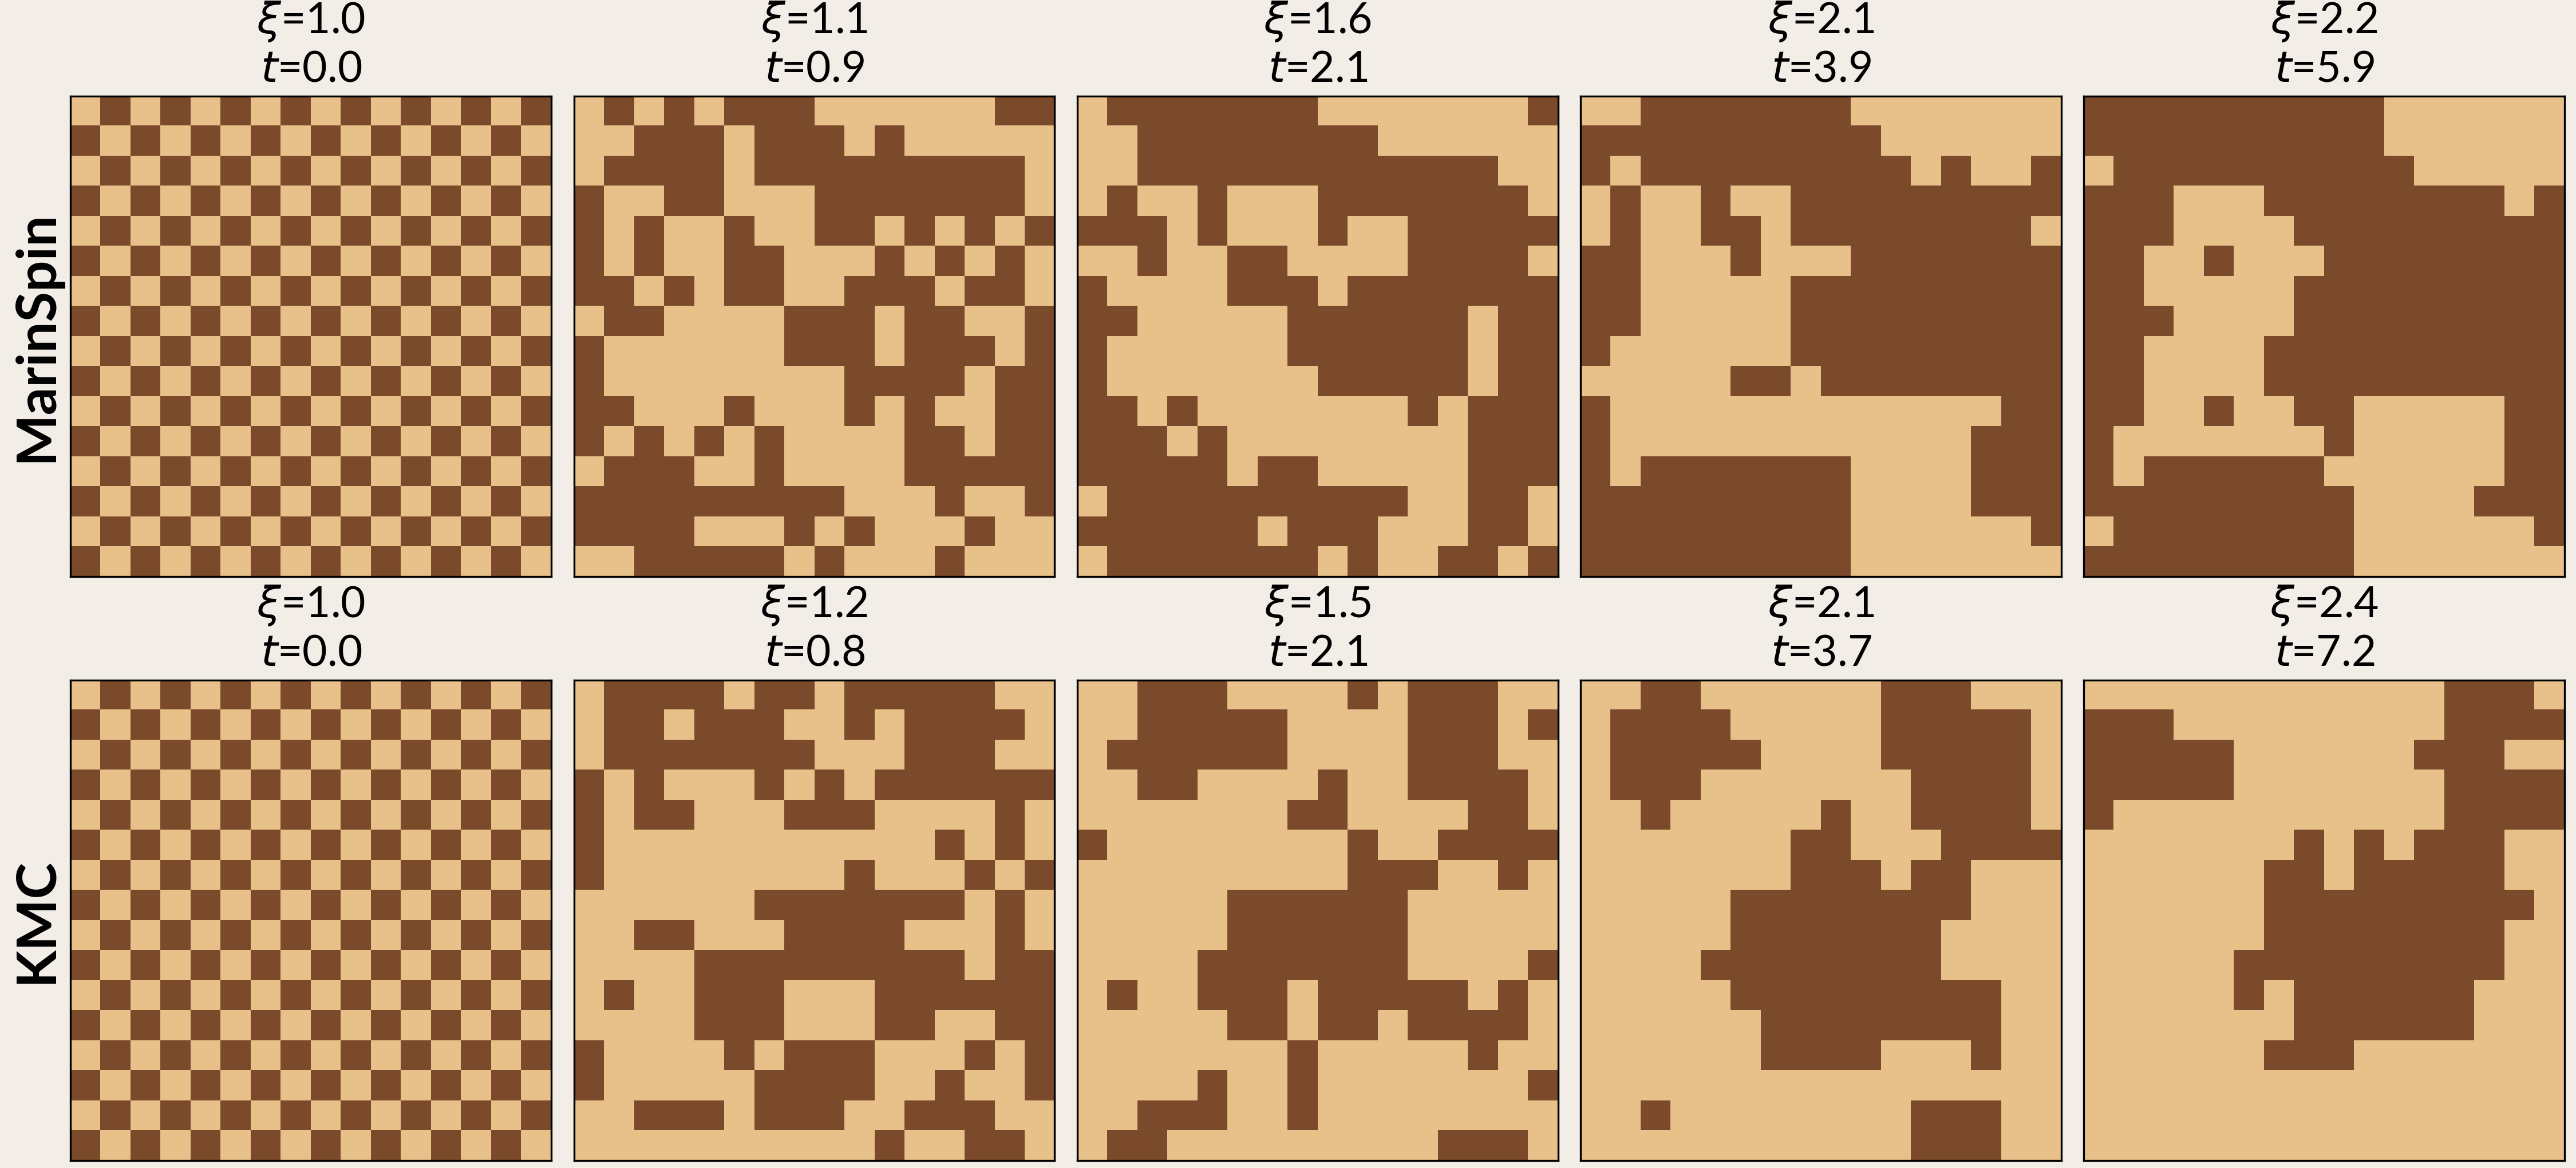
\includegraphics[width=\linewidth]{figures/quench_montage.png}\\[4pt]
    \raggedright
    MarinSpin (top) vs.\ KMC (bottom) from a checkerboard quench ($T{=}1.5$, sampling temp $0.9$);
    panels matched by \emph{event count}. Domains grow and $\xi$ rises together with KMC.
  \end{block}

\end{column}

% ======================= RIGHT COLUMN =======================================
\begin{column}{.48\paperwidth}

  \begin{block}{MarinSpin reproduces KMC behaviors with minimal additional loss}
    \centering
    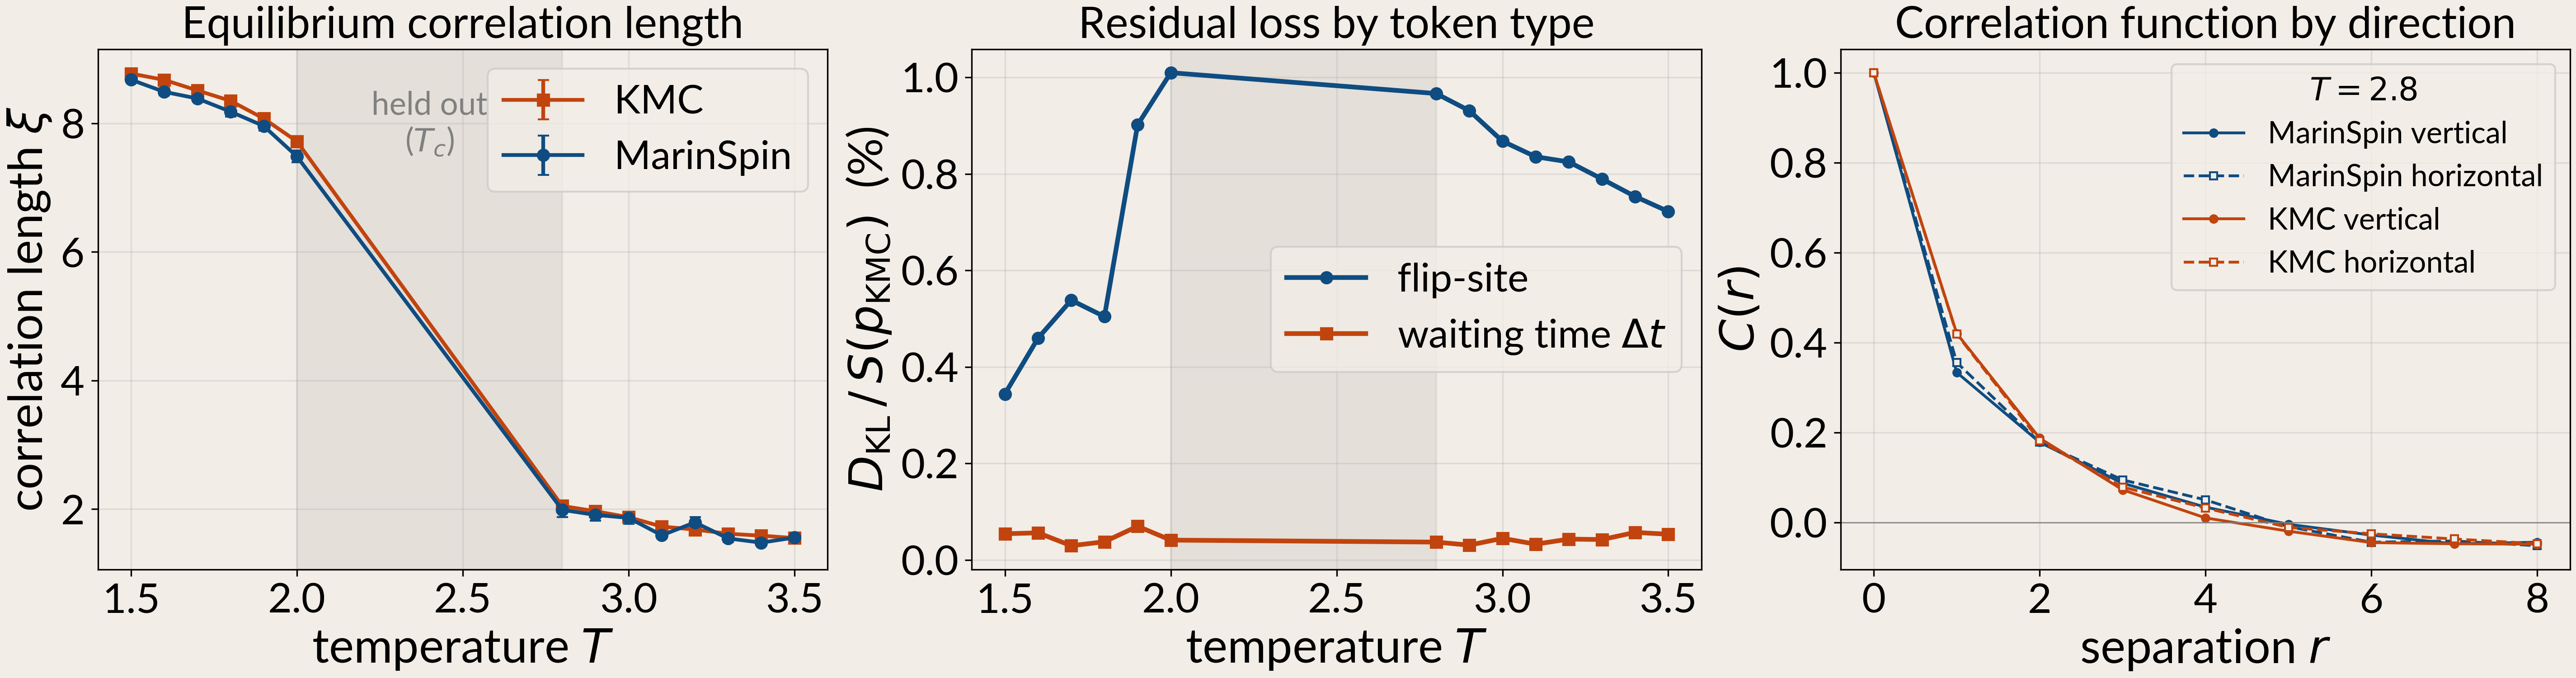
\includegraphics[width=\linewidth]{figures/triptych.png}\\[4pt]
    \raggedright
    The two-point correlation $C(r){=}\langle s_0 s_r\rangle$ measures how aligned two spins a
    distance $r$ apart are; the \keypt{correlation length} $\xi$ sets its decay,
    $C(r)\sim e^{-r/\xi}$.\par
    \keypt{Left:} equilibrium correlation length $\xi$ vs.\ $T$.\par
    \keypt{Middle:} residual $D_{\mathrm{KL}}/S(p_{\rm KMC})$ (\%).\par
    \keypt{Right:} the full $C(r)$ by direction (vertical vs.\ horizontal).
  \end{block}

  \begin{block}{MarinSpin learns the proper relative flip probabilities}
    \centering
    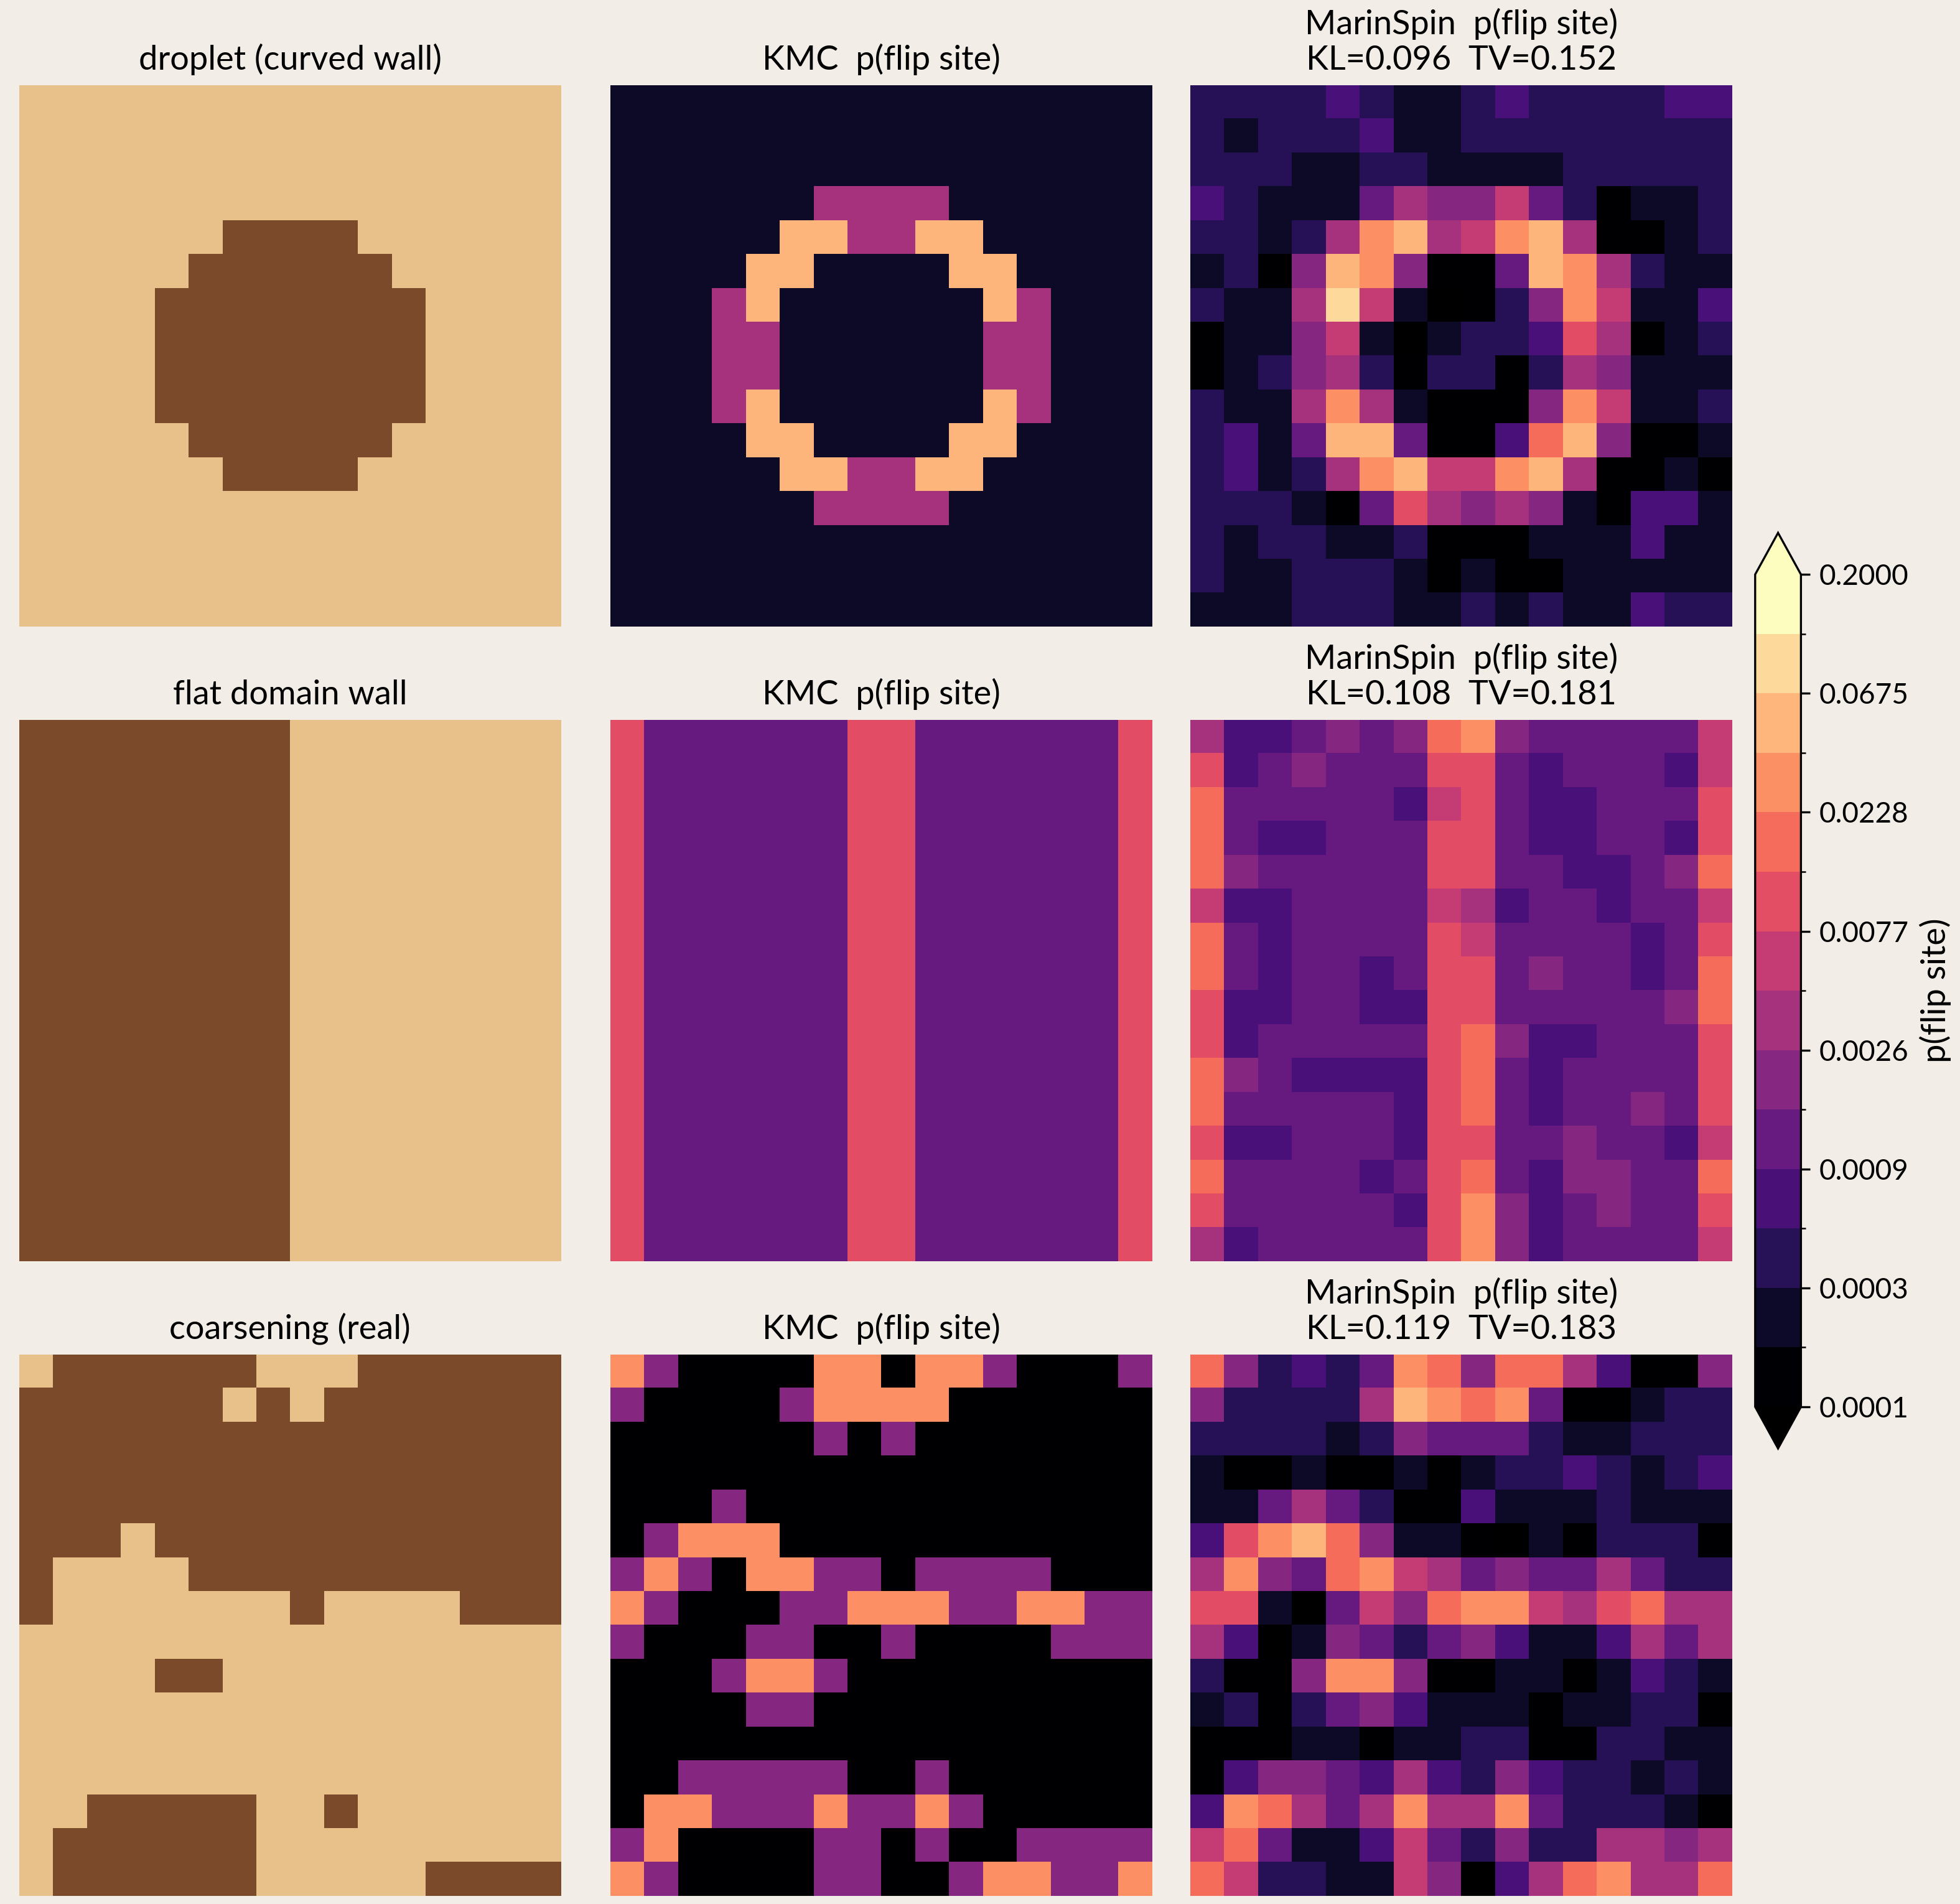
\includegraphics[width=0.95\linewidth]{figures/probs_cold.png}\\[4pt]
    \raggedright
    Per row: \keypt{spin config} $\to$ exact KMC $p$(flip) $\to$ model $p$(flip), $T{=}1.5$.\par
    $p$(flip site $i$) is the probability that site $i$ is the next to flip (KMC: $w_i/R$).
  \end{block}

  \begin{block}{Data, training \& prompt lessons}
    \begin{itemize}
      \item \textbf{Coverage:} more \emph{real} equilibrated data cuts per-step KL ($-$26\% cold,
            $-$37\% hot); the hot phase is coverage-limited.
      \item \textbf{Augmentation:} a limited trial of the 8 square symmetries (rotations/reflections,
            $D_4$) blurred the OOD flip probabilities, no clear benefit.
      \item \textbf{Prompt redundancy:} raster written \emph{twice}; dropping the copy
            \keypt{seemingly diverged the loss} (single trial).
      \item \textbf{Over-specialization:} longer training helps in-distribution KL but
            \emph{degrades} OOD fidelity.
      \item \textbf{Precision:} cold rate ratios span $\sim$200$\times$ --- \keypt{fp32 $\gg$ bf16}
            (32-bit floats capture more nuance in the parameter numbers than the coarser 16-bit bf16).
    \end{itemize}
  \end{block}

  \begin{block}{Next steps}
    \begin{itemize}
      \item \keypt{Continuous-$T$ encoding:} $T$ is currently a \emph{discrete} token, so MarinSpin
            can only simulate the exact trained temperatures. A continuous/embedded $T$ is the
            prerequisite for extending to the critical region.
      \item \keypt{v2 tokenization --- neighbor lists:} feed the lattice connectivity
            (edge / neighbor list) explicitly.
      \item Larger lattices; \keypt{conserved-order-parameter} dynamics.
    \end{itemize}
  \end{block}

  \begin{block}{References}
    {\footnotesize\setlength{\parskip}{0pt}
    \begin{minipage}[t]{0.49\linewidth}
    [1] Bortz \emph{et al.}, \emph{J. Comput. Phys.} 17, 10 (1975).\par
    [2] Metropolis \emph{et al.}, \emph{J. Chem. Phys.} 21, 1087 (1953).\par
    [3] Bray, \emph{Adv. Phys.} 43, 357 (1994).\par
    \end{minipage}\hfill
    \begin{minipage}[t]{0.49\linewidth}
    [4] Vaswani \emph{et al.}, \emph{NeurIPS} (2017).\par
    [5] Su \emph{et al.}, \emph{arXiv} 2104.09864 (2021).\par
    \end{minipage}
    }
  \end{block}

  \begin{block}{Acknowledgements}
    We thank \textbf{Antonia S.~J.~S.~Mey} and \textbf{Matteo T.~Degiacomi} (University of Edinburgh)
    for helpful discussions during the early stages of this work, and the
    \textbf{Google TPU Research Cloud (TRC)} for compute.
  \end{block}

\end{column}

\end{columns}
\end{frame}
\end{document}
